\documentclass[tikz, margin=3mm]{standalone}
\usepackage[colorlinks]{hyperref}

\usepackage{bbm}
\usepackage{amsmath}
\usepackage{amsfonts}
\usetikzlibrary{fit}
\usetikzlibrary{shapes.misc, positioning}
\usetikzlibrary{shapes}
\usetikzlibrary{arrows}
\usetikzlibrary{positioning}
\usetikzlibrary{calc}
\usetikzlibrary{decorations.pathreplacing}
\usetikzlibrary{decorations.pathmorphing}

\DeclareMathOperator*{\argmin}{arg\,min}
\newcommand{\Plus}{\mathord{
\begin{tikzpicture}[baseline=0ex, line width=3, scale=0.25]
\draw (1,0) -- (1,2);
\draw (0,1) -- (2,1);
\end{tikzpicture}}}

\newcommand{\PlusSmall}{\mathord{
\begin{tikzpicture}[baseline=0ex, line width=2, scale=0.10]
\draw (1,0) -- (1,2);
\draw (0,1) -- (2,1);
\end{tikzpicture}}}

\newcommand{\Minus}{\mathord{
\begin{tikzpicture}[baseline=0ex, line width=3, scale=0.25]
\draw (0,1) -- (2,1);
\end{tikzpicture}}}

\newcommand{\MinusSmall}{\mathord{\begin{tikzpicture}[baseline=0ex, line width=2, scale=0.10]
\draw (0,1) -- (2,1);
\end{tikzpicture}}}

\tikzset{weird fill/.style={append after command={
   \pgfextra
        \draw[sharp corners, fill=#1]% 
    (\tikzlastnode.west)% 
    [rounded corners=3pt] |- (\tikzlastnode.north)% 
    [rounded corners=1pt] -| (\tikzlastnode.east)% 
    [rounded corners=1pt] |- (\tikzlastnode.south)% 
    [rounded corners=3pt] -| (\tikzlastnode.west);
   \endpgfextra}}}





\begin{document}

 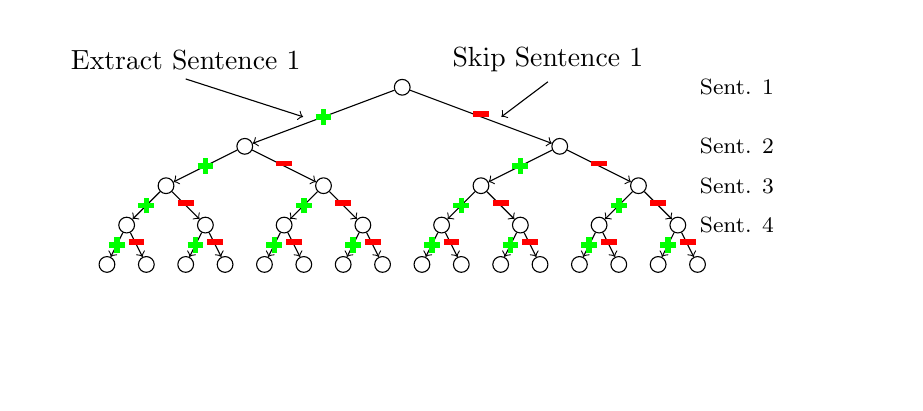
\begin{tikzpicture}
   \tikzstyle{sent}=[align=left]
   \tikzstyle{doc}=[rectangle,rounded corners,draw=black, very thick]



\node[draw,circle,minimum size=.20cm,inner sep=0pt] (a) at (0,0) {};
\node[draw,circle,minimum size=.20cm,inner sep=0pt] (b) at (.5,0) {};
\node[draw,circle,minimum size=.20cm,inner sep=0pt] (c) at (1,0) {};
\node[draw,circle,minimum size=.20cm,inner sep=0pt] (d) at (1.5,0) {};
\node[draw,circle,minimum size=.20cm,inner sep=0pt] (e) at (2,0) {};
\node[draw,circle,minimum size=.20cm,inner sep=0pt] (f) at (2.5,0) {};
\node[draw,circle,minimum size=.20cm,inner sep=0pt] (g) at (3,0) {};
\node[draw,circle,minimum size=.20cm,inner sep=0pt] (h) at (3.5,0) {};
\node[draw,circle,minimum size=.20cm,inner sep=0pt] (i) at (4,0) {};
\node[draw,circle,minimum size=.20cm,inner sep=0pt] (j) at (4.5,0) {};
\node[draw,circle,minimum size=.20cm,inner sep=0pt] (k) at (5,0) {};
\node[draw,circle,minimum size=.20cm,inner sep=0pt] (l) at (5.5,0) {};
\node[draw,circle,minimum size=.20cm,inner sep=0pt] (m) at (6,0) {};
\node[draw,circle,minimum size=.20cm,inner sep=0pt] (n) at (6.5,0) {};
\node[draw,circle,minimum size=.20cm,inner sep=0pt] (o) at (7,0) {};
\node[draw,circle,minimum size=.20cm,inner sep=0pt] (p) at (7.5,0) {};

\node[draw,circle,minimum size=.20cm,inner sep=0pt] (q) at (.25,.5) {};
\node[draw,circle,minimum size=.20cm,inner sep=0pt] (r) at (1.25,.5) {};
\node[draw,circle,minimum size=.20cm,inner sep=0pt] (s) at (2.25,.5) {};
\node[draw,circle,minimum size=.20cm,inner sep=0pt] (t) at (3.25,.5) {};
\node[draw,circle,minimum size=.20cm,inner sep=0pt] (u) at (4.25,.5) {};
\node[draw,circle,minimum size=.20cm,inner sep=0pt] (v) at (5.25,.5) {};
\node[draw,circle,minimum size=.20cm,inner sep=0pt] (w) at (6.25,.5) {};
\node[draw,circle,minimum size=.20cm,inner sep=0pt] (x) at (7.25,.5) {};

\node[draw,circle,minimum size=.20cm,inner sep=0pt] (y) at (.75,1) {};
\node[draw,circle,minimum size=.20cm,inner sep=0pt] (z) at (2.75,1) {};
\node[draw,circle,minimum size=.20cm,inner sep=0pt] (1) at (4.75,1) {};
\node[draw,circle,minimum size=.20cm,inner sep=0pt] (2) at (6.75,1) {};

\node[draw,circle,minimum size=.20cm,inner sep=0pt] (3) at (1.75,1.5) {};
\node[draw,circle,minimum size=.20cm,inner sep=0pt] (4) at (5.75,1.5) {};

\node[draw,circle,minimum size=.20cm,inner sep=0pt] (5) at (3.75,2.25) {};
\node[] at ($(x) + (.75,0)$) [] {\footnotesize Sent. 4};
\node[] at ($(x) + (.75,.5)$) [] {\footnotesize Sent. 3};
\node[] at ($(x) + (.75,1)$) [] {\footnotesize Sent. 2};
\node[] at ($(x) + (.75,1.75)$) [] {\footnotesize Sent. 1};

\draw[->] (5) -- (3); 
\draw[->] (5) -- (4);


\draw[->] (3) -- (y);
\draw[->] (3) -- (z);

\draw[->] (4) -- (1);
\draw[->] (4) -- (2);


\draw[->] (y) -- (q);
\draw[->] (y) -- (r);

\draw[->] (z) -- (s);
\draw[->] (z) -- (t);

\draw[->] (1) -- (u);
\draw[->] (1) -- (v);

\draw[->] (2) -- (w);
\draw[->] (2) -- (x);

\draw[->] (q) -- (a);
\draw[->] (q) -- (b);

\draw[->] (r) -- (c);
\draw[->] (r) -- (d);

\draw[->] (s) -- (e);
\draw[->] (s) -- (f);

\draw[->] (t) -- (g);
\draw[->] (t) -- (h);

\draw[->] (u) -- (i);
\draw[->] (u) -- (j);

\draw[->] (v) -- (k);
\draw[->] (v) -- (l);

\draw[->] (w) -- (m);
\draw[->] (w) -- (n);

\draw[->] (x) -- (o);
\draw[->] (x) -- (p);



\node (PA) at ($(5)!0.5!(3)$) [text=green]{$\PlusSmall$};
\node (MA) at ($(5)!0.5!(4)$) [text=red]{$\MinusSmall$};
\node at ($(3)!0.5!(y)$) [text=green]{$\PlusSmall$};
\node at ($(3)!0.5!(z)$) [text=red]{$\MinusSmall$};
\node at ($(4)!0.5!(1)$) [text=green]{$\PlusSmall$};
\node at ($(4)!0.5!(2)$) [text=red]{$\MinusSmall$};
\node at ($(y)!0.5!(q)$) [text=green]{$\PlusSmall$};
\node at ($(y)!0.5!(r)$) [text=red]{$\MinusSmall$};
\node at ($(z)!0.5!(s)$) [text=green]{$\PlusSmall$};
\node at ($(z)!0.5!(t)$) [text=red]{$\MinusSmall$};
\node at ($(1)!0.5!(u)$) [text=green]{$\PlusSmall$};
\node at ($(1)!0.5!(v)$) [text=red]{$\MinusSmall$};
\node at ($(2)!0.5!(w)$) [text=green]{$\PlusSmall$};
\node at ($(2)!0.5!(x)$) [text=red]{$\MinusSmall$};
\node at ($(q)!0.5!(a)$) [text=green]{$\PlusSmall$};
\node at ($(q)!0.5!(b)$) [text=red]{$\MinusSmall$};
\node at ($(r)!0.5!(c)$) [text=green]{$\PlusSmall$};
\node at ($(r)!0.5!(d)$) [text=red]{$\MinusSmall$};
\node at ($(s)!0.5!(e)$) [text=green]{$\PlusSmall$};
\node at ($(s)!0.5!(f)$) [text=red]{$\MinusSmall$};
\node at ($(t)!0.5!(g)$) [text=green]{$\PlusSmall$};
\node at ($(t)!0.5!(h)$) [text=red]{$\MinusSmall$};
\node at ($(u)!0.5!(i)$) [text=green]{$\PlusSmall$};
\node at ($(u)!0.5!(j)$) [text=red]{$\MinusSmall$};
\node at ($(v)!0.5!(k)$) [text=green]{$\PlusSmall$};
\node at ($(v)!0.5!(l)$) [text=red]{$\MinusSmall$};
\node at ($(w)!0.5!(m)$) [text=green]{$\PlusSmall$};
\node at ($(w)!0.5!(n)$) [text=red]{$\MinusSmall$};
\node at ($(x)!0.5!(o)$) [text=green]{$\PlusSmall$};
\node at ($(x)!0.5!(p)$) [text=red]{$\MinusSmall$};

\node (m1) at (1,2.6) {Extract Sentence 1};
\draw[->] (m1.south) -- (PA.west);
\node (m2) at (5.6,2.6) {Skip Sentence 1};
\draw[->] (m2.south) -- (MA.east);

   \draw[white] (-1,-1.5) rectangle (10,3);
\end{tikzpicture}
\end{document}
